
\section{Funkcje kształtu}
\label{sec:funkcje_ksztaltu}

Weźmy metalowy pręt o długości L. W punkcie \(x_1\) na pręcie przykładamy temperaturę \( T_1 \), a w punkcie \(x_2\) temperaturę \( T_2 \). Przewidujemy, że po nieskończenie długim czasie rozkład temperatury w pręcie pomiędzy tymi punktami będzie liniowy (Rys. \ref{fig:temperatura_pret}).

\begin{figure}[h]
\centering
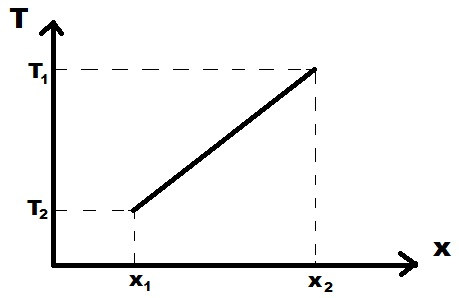
\includegraphics[width=10cm]{Zdjecia/3/rozklad_temperatury}
\caption{Temperatur pomiędzy punktami pręta}
\label{fig:temperatura_pret}
\end{figure}

Temperaturę pomiędzy tymi punktami możemy przedstawić funkcją \ref{eq:funkcja_liniowa}.

\begin{equation} \label{eq:funkcja_liniowa}
T(x)=a_0 + a_1 x, \quad dla \quad x \epsilon [x_1, x_2]
\end{equation}

Można wyznaczyć współczynniki funkcji liniowej mając dwa jej punty.

\begin{equation}
a_1 = \frac{T_2 - T_1}{x_2 - x_1}
\end{equation}

\begin{equation}
a_0 = T_2 - a_1 x_2
\end{equation}

Podstawiając współczyyniki do funkcji, możemy wyznaczyc funkcje kształtu.

\begin{equation}
T(x) = T_1 - \frac{T_2 - T_1}{L} x_1 + \frac{T_2 - T_1}{L} x = \frac{x_2 - x}{L}T_1 + \frac{x - x_1}{L}T_2 = N_1(x)T_1 + N_2(x)T_2
\end{equation}

gdzie
\begin{eqwhere}[2cm]
	\item[$N_1, N_2 $] funkcje kształtu.

\end{eqwhere}

Funkcje kształtu określają w jakim stopniu wartość temperatury z jednego węzła wpływa na wartość temperatury w dowolnym punkcie wewnątrz elementu. Dla większej liczby węzłów w jednowymiarowym elemencie funkcje kształtu są wielomianami wyższych rzędów. Poniżej znajduje się sposób wyznaczania funkcji kształtu na przykładzie 3-węzłowego elementu jednowymiarowego.

\begin{gather} \label{eq:interpolacja}
T(x) = a_0 + a_1 x + a_2 x^2 =
	\begin{bmatrix} 
	 	1 & x& x^2 \\
	\end{bmatrix}
	\begin{bmatrix} 
	 	a_0 \\
		a_1 \\
		a_2 \\
	\end{bmatrix} = \textbf{p} \textbf{a}^e = \textbf{N} \textbf{T}^e
\end{gather}

gdzie
\begin{eqwhere}[2cm]
	\item[$\textbf{p} $] wektor zmiennych kolejnych jednomianów T(x)
	\item[$\textbf{a}^e $] wektor współczynników kolejnych jednomianów T(x)
	\item[$\textbf{N} $] wektor funkcji kształtu
	\item[$\textbf{T}^e $] wektor wartości w węzłach.
\end{eqwhere}

Prawdziwe jest też poniższe równanie.

\begin{gather}
\textbf{T}^e =
	\begin{bmatrix} 
	 	1 & x_1& x_1^2 \\
		1 & x_2& x_2^2 \\
		1 & x_3& x_3^2 \\
	\end{bmatrix}
	\begin{bmatrix} 
	 	a_0 \\
		a_1 \\
		a_2 \\
	\end{bmatrix}
= \textbf{M}^e \textbf{a}^e
\end{gather}

Wyznaczając z tego równania \( \textbf{ a}^e  \) i podstawiając do równania \ref{eq:interpolacja}, otrzymamy następującą zależność.

\begin{equation}
\textbf{p a}^e = \textbf{p} {(\textbf{M}^e)}^{-1} \textbf{T}^e  = \textbf{N T}^e   \quad \Rightarrow \quad \textbf{N} = \textbf{p} {(\textbf{M}^e)}^{-1}
\end{equation}

Funkcje kształtu obliczone w taki sposób mają postać jak poniżej.

\begin{equation}
\begin{aligned}
N_1 = \frac{1}{det\textbf{M}^e} \big(x_2 x_3^2 - x_2^2 x_3 + (x_2^2 - x_3^2)x + (-x_2 + x_3)x^2\big) \\
N_2 = \frac{1}{det\textbf{M}^e} \big(x_1^2 x_3 - x_1 x_3^2 + (x_3^2 - x_1^2)x + (x_1 - x_3)x^2\big) \\
N_3 = \frac{1}{det\textbf{M}^e} \big(x_1 x_2^2 - x_1^2 x_2 + (x_1^2 - x_2^2)x + (-x_1 + x_2)x^2\big)
\end{aligned}
\end{equation}

Prawidłowo wyznaczone funkcje kształtu mają dwi ważną własności. Pierwsza związana jest z węzłami i mówi że każda funkcja przyjmuje wartość 1 w jednym węźle, a we wszystkich pozostałych 0. Druga własność mówi, że suma funkcji kształtu wewnątrz elmentu skończonego wynosi 1. Matematycznie zapisać te własności można następująco:

 \begin{equation} \label{eq:eq_zgodnosc}
	\left\{
                \begin{array}{ll}
		N_n(x_m, y_m) = 1, \quad dla \quad n=m \\
		N_n(x_m, y_m) = 0, \quad dla \quad \neq m 
                \end{array}
	\right.
 \end{equation}

 \begin{equation} \label{eq:WBS}
	\sum_1^n N_n = 1.
 \end{equation}






















